\documentclass[conference]{IEEEtran}
\IEEEoverridecommandlockouts
\usepackage{cite}
\usepackage{amsmath}
\usepackage{newtxtext,newtxmath}
\usepackage{graphicx}
\usepackage{booktabs}
\usepackage{multirow}
\usepackage{xcolor}
\usepackage{tikz}
\usetikzlibrary{positioning,arrows.meta,fit,calc}
\usepackage[hidelinks]{hyperref}
\graphicspath{{figures/}}

\begin{document}

\title{The Memory-Bandwidth Wall in Federated Learning Aggregation: Shared Memory, Threads, and Cache Tiling on Commodity CPUs}

\author{
\IEEEauthorblockN{Afaf Yunas\thanks{Roll numbers: Afaf Yunas (23L-0745), Kainat Asghar (23L-0687), Hussain Farhan (23L-2521). Code and experiment artifacts available at: \url{https://github.com/kainat-asghar/fl-aggregation-shared-memory}.}}
\IEEEauthorblockA{\textit{National University of Computer}\\
\textit{and Emerging Sciences (FAST-NU)}\\
Lahore, Pakistan\\
\texttt{younasafaf@gmail.com}}
\and
\IEEEauthorblockN{Kainat Asghar}
\IEEEauthorblockA{\textit{National University of Computer}\\
\textit{and Emerging Sciences (FAST-NU)}\\
Lahore, Pakistan\\
\texttt{kainat.bingo@gmail.com}}
\and
\IEEEauthorblockN{Hussain Farhan}
\IEEEauthorblockA{\textit{National University of Computer}\\
\textit{and Emerging Sciences (FAST-NU)}\\
Lahore, Pakistan\\
\texttt{muhammadhussainfarhan1@gmail.com}}
}

\maketitle

\begin{abstract}
In centralized federated learning (FL), the server must combine the model updates of every participating client in each round, and most frameworks perform this weighted average sequentially on a single core. We design, implement, and evaluate a multi-process aggregation scheme for commodity CPUs in which client updates are placed once in a \texttt{multiprocessing.shared\_memory} block and worker processes average disjoint slices of the model through zero-copy views. We compare it against a sequential FedAvg baseline, a multi-process variant that pickles and copies updates through pipes, and a multithreaded Numba kernel, all sharing one interface and one inner arithmetic kernel. On an AMD Ryzen 7 7735HS laptop (8 physical cores, 16 logical threads, 16\,GB single-channel DDR5, Windows 11, \texttt{spawn}), we sweep 10--1000 clients and models from 62K to 11.2M parameters. All 294 scheme/configuration pairs match the sequential result within $10^{-6}$, and FedAvg training on CIFAR-10 and FEMNIST reaches bit-identical accuracy with shared-memory aggregation. Shared-memory aggregation is 1.1--1.6$\times$ faster than sequential FedAvg once per-round update volume exceeds $\approx$12\,MB, but slower below that, where fixed coordination costs of 0.2--0.4\,ms dominate. Pickling-based multiprocessing is 5.6--21$\times$ slower than shared memory and never faster than the sequential baseline. Speedups stay far below linear because aggregation is memory-bandwidth bound: a STREAM-style measurement puts the sustained ceiling at 21\,GB/s, the single-core sequential kernel already reaches 9--12\,GB/s of it, and parallel efficiency therefore falls to 0.17--0.20 at eight workers. We further show that the cache tile used by the inner kernel must be sized for the \emph{aggregate} of all workers rather than for one: the conventional fixed 1\,MB tile overflows the shared last-level cache at four workers and above, costing up to 60\% of throughput and inverting the scaling curve, while a worker-count-aware tile restores monotone scaling at no cost to accuracy. In-process Numba threads were fastest in all 56 comparisons, so shared memory is the architecture of choice specifically where threads are not an option: GIL-bound, sandboxed, or separately deployed aggregator processes.
\end{abstract}

\begin{IEEEkeywords}
Federated Learning, FedAvg, Model Aggregation, Shared Memory, Multiprocessing, Parallel Computing, Memory Bandwidth, Cache Blocking, Roofline Model
\end{IEEEkeywords}

\section{Introduction}
Federated learning (FL) lets many distributed clients train a shared model without exposing their raw data: in every round, a central server collects client model updates and aggregates them into a new global model~\cite{mcmahan2017}. As FL deployments grow, two problems compound. First, most FL research is validated on small benchmarks that ignore the compute, network, and availability heterogeneity of real devices; FedScale showed that algorithm rankings can change once realistic traces are used~\cite{fedscale}. Second, the aggregation step itself becomes a systems bottleneck as participation grows.

In standard FedAvg, the server receives from each of $N$ clients an update vector of $P$ parameters and computes $g=\sum_{c} w_c\,u_c$. With $N$ in the hundreds and $P$ in the millions, this is $N\!\cdot\!P$ multiply-adds and $N\!\cdot\!P$ values streamed from memory per round, which many frameworks execute in a single process. Systems surveys note that optimization effort has concentrated on the client side (selection, compression, synchronization frequency), while server-side aggregation is comparatively under-studied~\cite{jiang2022}. Hardware solutions such as programmable switches and DPUs~\cite{gain,flagger} achieve large speedups but are unavailable on commodity servers, and existing shared-memory approaches~\cite{khan2023,lifl,falkor} each use shared memory differently and have not been compared like-for-like against a sequential baseline.

This paper studies whether multi-process shared-memory aggregation reduces aggregation latency on an ordinary multi-core CPU, at what client counts and model sizes the gains appear, and where they break down. We answer three research questions:
\begin{itemize}
\item \textbf{RQ1:} How does shared-memory aggregation compare with sequential FedAvg in aggregation time and speedup across client counts and model sizes?
\item \textbf{RQ2:} What does inter-process data movement (pickling and copying) cost compared with zero-copy shared memory?
\item \textbf{RQ3:} How do speedup and CPU utilization scale with worker count, and where do gains diminish?
\end{itemize}

Our contributions are: (i)~a controlled implementation of three aggregation schemes plus a Numba baseline behind one interface, sharing one arithmetic kernel, so that measured differences isolate the mechanism; (ii)~a benchmark sweep over 10--1000 clients, 62K--11.2M parameters, and 1--8 workers, with heavy-tailed client weights and simulated stragglers, together with a correctness study on real FedAvg training, all collected in a single uninterrupted run on one machine; (iii)~a roofline analysis, backed by a STREAM-style measurement of the same machine, showing that the gains are bounded by memory bandwidth and by the cost of placing updates into shared memory---on this platform a single core already draws half the available bandwidth, capping any parallel scheme near $2\times$; and (iv)~the identification of a cache-tiling pitfall specific to multi-process aggregation: the inner tile must be sized for the aggregate of all workers rather than for one, since the natural fixed 1\,MB tile overflows the shared last-level cache from four workers upward and converts a speedup into a slowdown, a defect invisible in any single-worker benchmark. Section~II reviews related work, Section~III presents the methodology, Section~IV the implementation and experimental setup, Section~V the results, and Section~VI concludes.

\section{Related Work}
Table~\ref{tab:related} summarizes the studies we reviewed. FedScale~\cite{fedscale} provides realistic FL datasets and a scalable runtime, and shows that benchmarks under-report real-world behavior. P2P-Fed~\cite{p2pfed} decentralizes aggregation over a Chord overlay. For the aggregation bottleneck itself, GAIN~\cite{gain} aggregates statelessly in programmable switches (up to 4.11$\times$ throughput, 86.5\% less traffic), and Flagger~\cite{flagger} uses DPUs and computational storage for encrypted cross-silo FL (436\% average acceleration). On commodity hardware, Khan et al.~\cite{khan2023} parallelize FedAvg across CPU cores with Numba (40--57\% less aggregation time) and observe that gains shrink as models grow; LIFL~\cite{lifl} passes updates between serverless aggregator functions through shared memory; and Falkor~\cite{falkor} accelerates secure-aggregation masking in GPU shared memory. The common pattern is that aggregation improves when computation is distributed and data movement is minimized, but no study compares these mechanisms against each other and a sequential baseline on an ordinary CPU under consistent metrics. That comparison is the gap this work addresses.

\begin{table}[t]
\caption{Summary of Reviewed Studies}
\label{tab:related}
\centering
\footnotesize
\setlength{\tabcolsep}{3pt}
\resizebox{\columnwidth}{!}{%
\begin{tabular}{@{}llll@{}}
\toprule
Study & System & Venue & Focus \\
\midrule
Lai et al.~\cite{fedscale} & FedScale & ICML'22 & Realistic FL benchmarking \\
Lim et al.~\cite{p2pfed} & P2P-Fed & CCGrid'25 & Decentralized Chord aggregation \\
Xia et al.~\cite{gain} & GAIN & ICDCS'24 & In-switch stateless aggregation \\
Pan et al.~\cite{flagger} & Flagger & ISCA'24 & DPU + storage, cross-silo FL \\
Jiang et al.~\cite{jiang2022} & Survey & IEEE TBD & FL systems optimization \\
Khan et al.~\cite{khan2023} & Numba agg. & IEEE'23 & Multi-core CPU aggregation \\
Qi et al.~\cite{lifl} & LIFL & MLSys'24 & Shared-memory serverless FL \\
Belorgey et al.~\cite{falkor} & Falkor & WAHC'23 & GPU secure-aggregation masking \\
\bottomrule
\end{tabular}}
\end{table}

\section{Research Methodology}
\label{sec:method}
We follow an experimental, quantitative methodology. All schemes implement one interface, \texttt{aggregate(U, w)}~$\rightarrow g$, where $U\in\mathbb{R}^{N\times P}$ holds the float32 client updates and $w_c=n_c/\sum_j n_j$ are weights normalized by client dataset size, so no final division is needed. Every scheme calls the same inner NumPy kernel, so any measured difference comes from the aggregation mechanism rather than from different arithmetic. Fig.~\ref{fig:schemes} illustrates the three schemes.

\begin{figure*}[t]
\centering
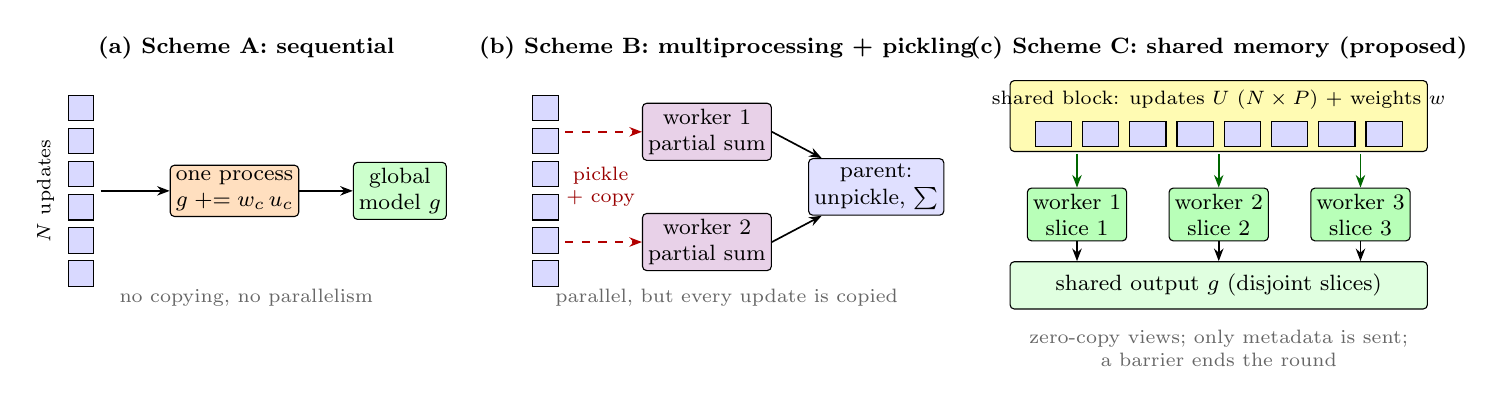
\begin{tikzpicture}[
  font=\footnotesize,
  box/.style={draw, rounded corners=1.5pt, minimum height=6mm, inner sep=2pt, align=center},
  upd/.style={draw, fill=blue!15, minimum width=3.2mm, minimum height=3.2mm, inner sep=0pt},
  arr/.style={-{Stealth[length=1.6mm]}, semithick},
  ttl/.style={font=\footnotesize\bfseries, anchor=south}]
% ---------------- (a) sequential
\node[ttl] at (2.4,3.05) {(a) Scheme A: sequential};
\foreach \i in {0,...,5} \node[upd] at (0.3,2.55-\i*0.42) {};
\node[font=\scriptsize, rotate=90] at (-0.15,1.5) {$N$ updates};
\node[box, fill=orange!25] (ap) at (2.25,1.5) {one process\\$g \mathrel{+}= w_c\,u_c$};
\draw[arr] (0.55,1.5) -- (ap.west);
\node[box, fill=green!20] (ag) at (4.35,1.5) {global\\model $g$};
\draw[arr] (ap) -- (ag);
\node[font=\scriptsize, text=black!60] at (2.4,0.15) {no copying, no parallelism};
% ---------------- (b) pickling
\begin{scope}[xshift=5.9cm]
\node[ttl] at (2.6,3.05) {(b) Scheme B: multiprocessing + pickling};
\foreach \i in {0,...,5} \node[upd] at (0.3,2.55-\i*0.42) {};
\node[box, fill=violet!18] (w1) at (2.35,2.25) {worker 1\\partial sum};
\node[box, fill=violet!18] (w2) at (2.35,0.85) {worker 2\\partial sum};
\draw[arr, red!70!black, dashed] (0.55,2.25) -- (w1.west);
\draw[arr, red!70!black, dashed] (0.55,0.85) -- (w2.west);
\node[font=\scriptsize, text=red!60!black, align=center] at (1.0,1.55) {pickle\\+ copy};
\node[box, fill=blue!12] (bp) at (4.5,1.55) {parent:\\unpickle, $\sum$};
\draw[arr] (w1.east) -- (bp);
\draw[arr] (w2.east) -- (bp);
\node[font=\scriptsize, text=black!60] at (2.6,0.15) {parallel, but every update is copied};
\end{scope}
% ---------------- (c) shared memory
\begin{scope}[xshift=12.0cm]
\node[ttl] at (2.75,3.05) {(c) Scheme C: shared memory (proposed)};
\node[box, fill=yellow!30, minimum width=5.3cm, minimum height=9mm] (shm) at (2.75,2.45) {};
\node[font=\scriptsize, anchor=north] at (shm.north) {shared block: updates $U$ ($N\times P$) + weights $w$};
\foreach \i in {0,...,7} \node[upd, minimum width=4.6mm] at (0.65+\i*0.6,2.22) {};
\foreach \k/\x in {1/0.95,2/2.75,3/4.55} {
  \node[box, fill=green!28] (c\k) at (\x,1.2) {worker \k\\slice \k};
  \draw[arr, green!40!black] (\x,1.97) -- (c\k.north);
}
\node[box, fill=green!12, minimum width=5.3cm] (out) at (2.75,0.3) {shared output $g$ (disjoint slices)};
\foreach \k in {1,2,3} \draw[arr] (c\k.south) -- (c\k.south |- out.north);
\node[font=\scriptsize, text=black!60, align=center] at (2.75,-0.5) {zero-copy views; only metadata is sent;\\a barrier ends the round};
\end{scope}
\end{tikzpicture}
\caption{The three aggregation schemes: (a) sequential baseline; (b) multiprocessing with explicit pickling, where client chunks are serialized and copied to each worker; (c) multiprocessing with zero-copy shared memory and slice partitioning, where workers read the shared update block directly and write disjoint slices of the output.}
\label{fig:schemes}
\end{figure*}

\subsection{Aggregation Schemes}
\textbf{Scheme A (sequential FedAvg).} A single process accumulates $g \mathrel{+}= w_c u_c$ over all clients, with no inter-process communication and no parallelism.

\textbf{Scheme B (multiprocessing with pickling).} A persistent pool of $W$ worker processes is created once. The parent partitions clients into $W$ contiguous chunks and sends each worker its chunk of full update tensors, explicitly serialized with \texttt{pickle} and copied through a pipe. Each worker returns a pickled partial sum, and the parent adds the $W$ partial vectors. This scheme parallelizes the arithmetic but pays serialization and copying costs that grow with $N\!\cdot\!P$, so it isolates the cost of data movement.

\textbf{Scheme C (multiprocessing with shared memory, proposed).} The parent allocates one shared-memory block holding $U$ followed by $w$, and a second shared block for the $P$-value output. Workers receive only metadata (block names, $N$, $P$, partition mode, worker index), attach zero-copy NumPy views, and write their results straight into the output buffer. A barrier signals the parent that all writes are complete.

\textbf{Numba baseline.} To reproduce Khan et al.~\cite{khan2023}, we add an in-process multithreaded Numba~\cite{numba} kernel that tiles the parameter vector across $W$ threads.

\subsection{Work Partitioning}
Scheme C supports two partitioning strategies. In \emph{slice partitioning} (default), worker $k$ averages a contiguous slice of the $P$ parameters over all $N$ clients; each worker streams a contiguous memory region and writes a disjoint part of the output, so no locks and no final reduction are needed. Slice boundaries are aligned to 64-byte cache lines to avoid false sharing. In \emph{client partitioning}, each worker sums a disjoint subset of clients over the full vector into a shared $W\times P$ partial buffer, and the parent reduces the $W$ rows. We expected client partitioning to suit large $N$ and slice partitioning to suit large $P$.

\subsection{Correctness and Realism}
Floating-point summation order differs between schemes, so we require numerical equivalence rather than bitwise identity: before any timing, every scheme's output is checked against Scheme A with \texttt{allclose(atol=1e-6)}. In real FedAvg training, we further require that all schemes produce the same accuracy trajectory. To approximate FedScale-style heterogeneity, client dataset sizes are drawn from a heavy-tailed log-normal distribution and determine the weights. Straggler delays are simulated on a virtual clock (arrival time = data size $\times$ log-normal device speed + log-normal network delay); updates are aggregated in arrival order, and the delay is recorded but excluded from the measured aggregation time, which models update arrival rather than aggregation cost.

\subsection{Hypotheses}
We formulate three core hypotheses grounded in parallel systems principles:
\begin{itemize}
\item \textbf{H1 (Shared-Memory Scaling):} Multi-process shared-memory aggregation (Scheme C) outperforms sequential aggregation (Scheme A), with speedup increasing with client count $N$ and parameter count $P$ up to a plateau.
\emph{Rationale:} Dividing $N\cdot P$ arithmetic operations across $W$ processes reduces CPU time with negligible IPC overhead once update volume exceeds the sub-millisecond coordination threshold.
\item \textbf{H2 (Cost of Serialization):} Shared memory substantially outperforms pickling-based multiprocessing (Scheme B), with the performance margin expanding as model size grows.
\emph{Rationale:} Scheme B incurs $O(N\cdot P)$ memory allocations and serialization copies through OS pipes that serialize on the parent process, whereas Scheme C maps physical memory pages directly into worker address spaces without data movement.
\item \textbf{H3 (Bandwidth Saturation):} Speedup plateaus beyond an optimal worker count due to memory-bandwidth contention rather than synchronization overhead.
\emph{Rationale:} FL aggregation exhibits low arithmetic intensity ($1/4$ FLOP/byte). Multiple concurrent worker cores saturate the DRAM bandwidth subsystem, causing memory stalls to outpace compute gains.
\end{itemize}

\section{Implementation and Experimental Setup}
\subsection{Implementation Details}
All schemes are implemented in Python with NumPy~\cite{numpy} and the standard \texttt{multiprocessing} and \texttt{multiprocessing.shared\_memory} modules~\cite{pyshm}. Key decisions are:

\textit{Common kernel.} The inner kernel walks the parameter vector in tiles and, inside each tile, loops over clients in order. Each update byte is therefore read from DRAM once and the accumulator stays in cache, which makes the sequential baseline as cache-friendly as a parallel slice; speedups are not an artifact of cache effects. Because each element is summed in the same client order, Scheme C with slice partitioning is bit-identical to Scheme A. BLAS libraries are pinned to one thread in every process, so Scheme A genuinely uses one core.

The tile size is not a free constant. Each worker keeps two tile-sized buffers hot (its slice of the accumulator and a scratch vector), so $W$ workers occupy $W\!\cdot\!2\!\cdot\!\textit{tile}$ bytes of the shared last-level cache. We therefore derive the tile from the worker count rather than fixing it: the implementation budgets a quarter of the detected LLC for the workers' tiles, $W\!\cdot\!2\!\cdot\!\textit{tile}\le\text{LLC}/4$, clamped to $[64\,\text{KB},1\,\text{MB}]$ and capped at the length of the slice itself, so a model smaller than one tile is processed in a single untiled pass exactly as before. Section~\ref{sec:rq3} measures what the conventional fixed 1\,MB tile costs instead. The tile affects only the traversal order of memory, never the arithmetic, so results are bitwise independent of it.

\textit{Persistent pools.} Workers are created once per worker count and reused across rounds, so process start-up is measured separately and never counted inside a round. Workers attach to shared blocks once and cache the handle.

\textit{Bounded pickling.} Scheme B streams each worker's chunk in pickled batches of at most 64\,MB, sent round-robin so workers compute while the parent pickles the next batch. Total bytes copied are unchanged; batching only bounds peak memory on a 16\,GB machine.

\textit{Synchronization and release.} A barrier with $W\!+\!1$ parties (the workers and the parent) marks the end of each round. Workers detach before the parent closes and unlinks a block, which is required on Windows, where a block is freed only when its last handle closes.

\textit{FL simulation.} The correctness track uses a lightweight FedAvg loop written directly in PyTorch~\cite{pytorch} instead of Flower~\cite{flower}, so that our aggregators are called directly and the comparison stays controlled.

\subsection{Datasets and Models}
\textit{Correctness track.} We train LeNet-5~\cite{lenet} (62,006 parameters for CIFAR-10, 66,126 for FEMNIST) with 20 clients for 20 rounds (one local epoch, SGD with learning rate 0.01, momentum 0.9, batch size 32). CIFAR-10~\cite{cifar} is split non-IID with a Dirichlet label distribution, $\alpha=0.5$~\cite{hsu2019}, giving 1,079--4,614 samples per client. For FEMNIST (LEAF~\cite{leaf}), each client is a group of 10 real writers (1,570--2,406 samples), with a per-writer 90/10 train/test split. Each dataset is trained once per scheme with the same seed, initial model, data split, and arrival order, so the aggregator is the only difference between runs.

\textit{Scalability track.} Aggregation time depends on update size and client count, not on data content, so we generate random float32 updates at real model sizes (Table~\ref{tab:models}): LeNet-5, MobileNetV2~\cite{mobilenetv2} (3,504,872 parameters), and ResNet-18~\cite{resnet} with a 10-class head (11,173,962 parameters). Updates are generated directly into the shared block, and Schemes A and B read the same memory, so no duplicate copy exists. The raw update block is capped at 3.5\,GiB, which determines the largest client count for each model.

\begin{table}[t]
\caption{Model Sizes and Client Counts}
\label{tab:models}
\centering
\footnotesize
\setlength{\tabcolsep}{3.5pt}
\resizebox{\columnwidth}{!}{%
\begin{tabular}{@{}lrrll@{}}
\toprule
Model & Params & Update & Clients $N$ & Max block \\
\midrule
LeNet-5 & 62,006 & 0.25\,MB & 10, 50, 100, 250, 500, 1000 & 0.23\,GiB \\
MobileNetV2 & 3.50M & 14.0\,MB & 10, 50, 100, 250 & 3.26\,GiB \\
ResNet-18 & 11.17M & 44.7\,MB & 10, 25, 50, 75 & 3.12\,GiB \\
\bottomrule
\end{tabular}}
\end{table}

\subsection{Hardware and Software}
All experiments ran on one commodity laptop (Table~\ref{tab:env}) on mains power, under the Windows ``High performance'' power plan, with background applications closed. The AMD Ryzen 7 7735HS has eight physical cores with SMT (16 logical threads). Its 16\,GB of DDR5-4800 is supplied by a single memory module, so the machine is effectively single-channel; Section~\ref{sec:rq3} shows that this, and not the core count, is what bounds every result in this paper. Windows starts worker processes with \texttt{spawn}, so each worker re-imports the interpreter rather than inheriting the parent's address space as \texttt{fork} would on Linux. Because the pools are created once and reused for every round (Section~\ref{sec:e2e}), this affects start-up cost only, not per-round time.

\begin{table}[t]
\caption{Hardware and Software Environment}
\label{tab:env}
\centering
\footnotesize
\resizebox{\columnwidth}{!}{%
\begin{tabular}{@{}ll@{}}
\toprule
Component & Specification \\
\midrule
CPU & AMD Ryzen 7 7735HS, 8 physical cores (16 logical, SMT, up to 4.75\,GHz) \\
Memory & 16\,GB DDR5-4800, single module (single-channel) \\
Measured bandwidth & 16--19\,GB/s (STREAM copy/add/triad), 27\,GB/s (streaming read) \\
OS / start method & Windows 11 Pro 26200 (x86-64), \texttt{spawn} \\
Software & Python 3.12.10, NumPy 2.5.4 (OpenBLAS), psutil 7.2.2, \\
 & Numba 0.68.1, PyTorch 2.15.0+cpu \\
\bottomrule
\end{tabular}}
\end{table}

\subsection{Metrics and Protocol}
We report wall-clock aggregation time per round (from all updates being available until the global model is ready), speedup over Scheme A, parallel efficiency (speedup$/W$), and CPU utilization as busy cores (process-tree CPU-seconds per wall-second). For Scheme C we report compute-only time (updates already resident in shared memory) and end-to-end time, which adds the parent writing all $N$ updates into the block. Workers $W\in\{1,2,4,8\}$, chosen to span one worker up to the eight physical cores. For each configuration, one discarded warm-up run per scheme (which also performs the correctness check) is followed by 10 timed repetitions, interleaved across schemes in shuffled order to spread thermal drift, with garbage collection disabled inside each timed call. We report medians and inter-quartile ranges; the whole sweep is a single uninterrupted run on one machine, and no configuration was re-run or discarded. Across all 294 measured pairs the inter-quartile range was a median of 3.3\% of the median time (90th percentile 14.9\%). CPU and memory are sampled in a separate instrumented pass so that the sampler never perturbs the timings.

\section{Results}
\subsection{Correctness}
\label{sec:correctness}
All 294 scheme/configuration pairs of the scalability sweep passed the \texttt{allclose} check against Scheme A; the largest absolute difference was $5.6\times10^{-9}$. In FedAvg training (Fig.~\ref{fig:fl}, Table~\ref{tab:fl}), Scheme C produced exactly the same global model as Scheme A in every round, and therefore identical accuracy: 53.58\% on CIFAR-10 and 80.20\% on FEMNIST after 20 rounds. Scheme B sums in a different order; its parameters differ by at most $1.2\times10^{-7}$ and its accuracy by at most 0.32 percentage points, attributable to floating-point summation order. All schemes are therefore functionally equivalent, and the timing comparisons below are like-for-like.

Bit-identity is a property of the partitioning, not of the tile size. Within a tile every output element still accumulates clients in the fixed order $0\ldots N\!-\!1$, so changing the tile---as the worker-count-aware rule of Section~\ref{sec:rq3} does---cannot change the result. We verified this explicitly: tiles of 64\,KB, 256\,KB, 1\,MB and 4\,MB produce bitwise equal output.

\begin{figure}[t]
\centering
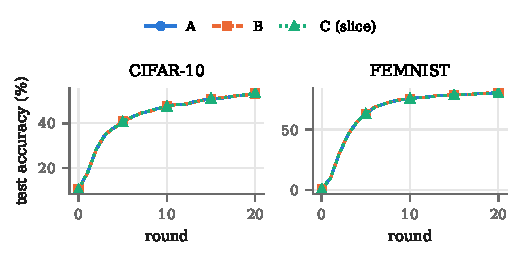
\includegraphics[width=\columnwidth]{fig_fl}
\caption{Test accuracy of FedAvg with each aggregation scheme (20 clients). The curves of A and C coincide exactly; B differs by at most 0.32 percentage points. At this scale (20 clients, 0.25\,MB updates) the round is far below the break-even point of Section~\ref{sec:rq1}, so Scheme C is slower than Scheme A in wall-clock terms here; this figure concerns equivalence, not speed.}
\label{fig:fl}
\end{figure}

\begin{table}[t]
\caption{Federated Training Results (20 Clients, 20 Rounds, $W=4$)}
\label{tab:fl}
\centering
\footnotesize
\setlength{\tabcolsep}{4pt}
\resizebox{\columnwidth}{!}{%
\begin{tabular}{@{}llrrrr@{}}
\toprule
Dataset & Scheme & Final acc. & Max $|\Delta\text{acc}|$ & Max $|\Delta g|$ & Agg. time \\
\midrule
\multirow{3}{*}{CIFAR-10} & A & 53.58\% & -- & -- & 0.49\,ms \\
 & B & 53.26\% & 0.32\,pp & $8.9\!\times\!10^{-8}$ & 5.81\,ms \\
 & C & 53.58\% & 0.00\,pp & 0 & 1.38\,ms \\
\midrule
\multirow{3}{*}{FEMNIST} & A & 80.20\% & -- & -- & 0.54\,ms \\
 & B & 80.00\% & 0.26\,pp & $1.2\!\times\!10^{-7}$ & 5.96\,ms \\
 & C & 80.20\% & 0.00\,pp & 0 & 1.48\,ms \\
\bottomrule
\end{tabular}}
\end{table}

\subsection{RQ1: Aggregation Time and Speedup}
\label{sec:rq1}
Fig.~\ref{fig:time} and Table~\ref{tab:main} show aggregation time as the number of clients grows, with $W=4$ for the parallel schemes. We report $W=4$ because it is the measured optimum for every model on this machine, not merely the core count divided by two; Section~\ref{sec:rq3} gives the full sweep over $W$ and explains why the optimum sits below the eight physical cores. Aggregation time grows almost linearly with $N\!\cdot\!P$ for all schemes.

Shared-memory aggregation with slice partitioning is faster than sequential FedAvg in 13 of 14 configurations, by 1.09--1.64$\times$ once the work is non-trivial. For ResNet-18 with 75 clients, the round time falls from 274\,ms to 207\,ms. The break-even point is small models with few clients: for LeNet with 10 clients, Scheme C takes 0.59\,ms against 0.23\,ms for Scheme A, because dispatching metadata and waiting at the barrier costs a fixed 0.2--0.4\,ms that exceeds the arithmetic. LeNet reaches break-even at about 50 clients, i.e.\ 12\,MB of updates, which is the same threshold we observe for the larger models when expressed in bytes rather than clients. Unlike in a compute-bound workload, the speedup saturates quickly with update volume rather than continuing to grow: it rises from 1.09$\times$ at 12\,MB to 1.64$\times$ at 236\,MB for LeNet, but only from 1.26$\times$ to 1.37$\times$ across the entire 134--3342\,MB range of MobileNetV2. Section~\ref{sec:rq3} attributes this ceiling to memory bandwidth.

The multithreaded Numba baseline was the fastest scheme in \emph{all} 56 scheme/worker comparisons (e.g., 122\,ms vs.\ 207\,ms for ResNet-18 at $N=75$; 128\,ms vs.\ 205\,ms for MobileNetV2 at $N=250$), because threads in one process need neither inter-process signalling nor a barrier across processes, and because they share one address space and therefore one set of page tables when streaming the update block. That threads win outright does not weaken the case for Scheme C so much as locate it: shared memory is the right choice precisely when threads are unavailable, and within pure Python multiprocessing it is unambiguously the best option, as the next section shows. It does, however, mean that a deployment free to use compiled multithreaded kernels should do so.

\begin{figure*}[t]
\centering
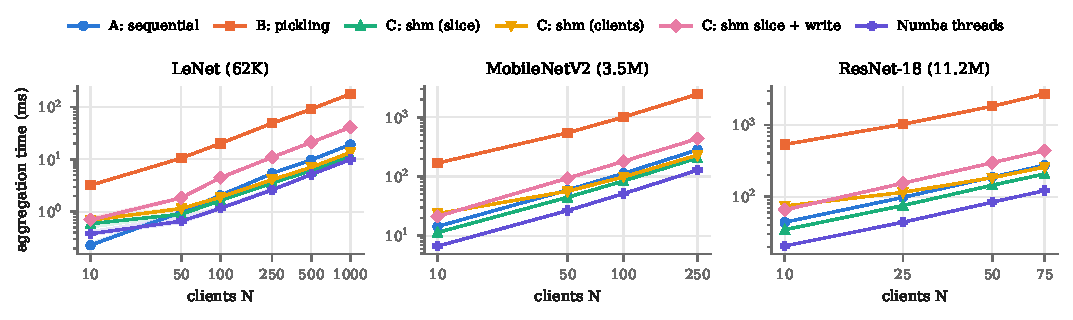
\includegraphics[width=\textwidth]{fig_time}
\caption{Median aggregation time per round vs.\ client count ($W=4$ for parallel schemes; bands show the inter-quartile range). Note the logarithmic axes.}
\label{fig:time}
\end{figure*}

\begin{table*}[t]
\caption{Median Aggregation Time per Round in ms ($W=4$, the optimum on this machine) and Speedup of Scheme C (Slice) over Scheme A}
\label{tab:main}
\centering
\footnotesize
\begin{tabular}{@{}lrrrrrrrrrr@{}}
\toprule
Model & $N$ & Data (MB) & A: sequential & B: pickling & C: slice & C: clients & C: slice + write & Numba & Speedup C/A & B/C \\
\midrule
\multirow{6}{*}{LeNet-5}
 & 10 & 2 & 0.23 & 3.19 & 0.59 & 0.69 & 0.70 & 0.38 & 0.39$\times$ & 5.4$\times$ \\
 & 50 & 12 & 0.98 & 10.51 & 0.90 & 1.15 & 1.84 & 0.66 & 1.09$\times$ & 11.7$\times$ \\
 & 100 & 24 & 2.05 & 20.07 & 1.64 & 1.90 & 4.47 & 1.17 & 1.25$\times$ & 12.3$\times$ \\
 & 250 & 59 & 5.40 & 48.70 & 3.53 & 4.09 & 10.94 & 2.60 & 1.53$\times$ & 13.8$\times$ \\
 & 500 & 118 & 9.76 & 90.77 & 6.09 & 7.03 & 21.07 & 5.15 & 1.60$\times$ & 14.9$\times$ \\
 & 1000 & 236 & 19.09 & 176.44 & 11.64 & 13.46 & 40.92 & 9.89 & 1.64$\times$ & 15.2$\times$ \\
\midrule
\multirow{4}{*}{MobileNetV2}
 & 10 & 134 & 14.30 & 168.65 & 11.31 & 23.51 & 21.19 & 6.64 & 1.26$\times$ & 14.9$\times$ \\
 & 50 & 668 & 58.86 & 546.90 & 44.43 & 56.35 & 93.48 & 26.50 & 1.32$\times$ & 12.3$\times$ \\
 & 100 & 1337 & 112.86 & 1009.04 & 83.85 & 98.21 & 180.19 & 51.23 & 1.35$\times$ & 12.0$\times$ \\
 & 250 & 3342 & 281.48 & 2454.17 & 205.21 & 229.75 & 435.64 & 127.73 & 1.37$\times$ & 12.0$\times$ \\
\midrule
\multirow{4}{*}{ResNet-18}
 & 10 & 426 & 43.95 & 536.61 & 34.57 & 73.94 & 65.52 & 20.49 & 1.27$\times$ & 15.5$\times$ \\
 & 25 & 1066 & 97.64 & 1026.10 & 75.16 & 114.90 & 153.88 & 43.92 & 1.30$\times$ & 13.7$\times$ \\
 & 50 & 2131 & 187.54 & 1829.02 & 144.62 & 183.98 & 298.07 & 83.72 & 1.30$\times$ & 12.6$\times$ \\
 & 75 & 3197 & 274.40 & 2719.53 & 207.47 & 258.49 & 439.21 & 121.55 & 1.32$\times$ & 13.1$\times$ \\
\bottomrule
\end{tabular}
\end{table*}

\subsection{RQ2: Cost of Data Movement}
Pickling-based multiprocessing (Scheme B) was the slowest scheme in every configuration, 5.6--21$\times$ slower than Scheme C (Fig.~\ref{fig:copy}a) and 8.7--17$\times$ slower than the sequential baseline. The gap is 5.4$\times$ for 2\,MB of updates and widens with model size, to 12--15$\times$ for LeNet from 59\,MB upwards and 12--16$\times$ for MobileNetV2 and ResNet-18. Fig.~\ref{fig:copy}b explains why: Scheme B moves data at only 0.7--1.4\,GB/s, while the sequential kernel sustains 9.1--12.1\,GB/s, Scheme C up to 19.8\,GB/s and the Numba baseline up to 26.6\,GB/s. Pickling copies every update at least twice (into the pickle buffer, and through the pipe into the worker's heap) and is performed by the parent alone. Adding workers therefore does not help and can hurt: for ResNet-18 at $N=75$, Scheme B takes 2.86\,s with one worker and 3.25\,s with eight, while its process tree keeps only 2.0--3.4 cores busy, most of that the parent serializing (Fig.~\ref{fig:scaling}). Copying overhead dominates at every update size we tested, so zero-copy sharing is a prerequisite, not an optimization, for multi-process aggregation in Python.

The ratio B/C should be read with care, because it compresses on a bandwidth-limited machine: Scheme C is itself held back here, which enlarges the denominator. The absolute figure is the robust one. Scheme B sustains 0.7--1.4\,GB/s regardless of model or worker count, an order of magnitude below every other scheme, because it is bound by serialization and pipe copies rather than by the memory system---and that bound is a property of the mechanism, not of this CPU.

Pickling also incurs an unsustainable memory footprint. The combined resident set size (RSS) of the parent and workers grew by up to 1.3\,GB above idle under Scheme B, due to duplicated serialized byte arrays in transit and in worker heaps, with the peak at ResNet-18 ($N=75$). In contrast, Scheme C required no measurable auxiliary heap memory at all (0\,MB above idle in every configuration), as all workers map zero-copy views directly into the single shared update block.

\begin{figure}[t]
\centering
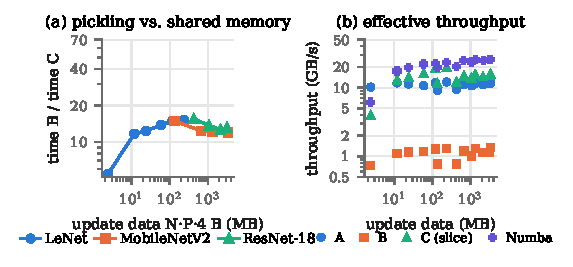
\includegraphics[width=\columnwidth]{fig_copy}
\caption{(a) Slowdown of pickling (B) relative to shared memory (C) at $W=4$, by total update size. (b) Effective throughput (update bytes processed per second) of each scheme, against the 21\,GB/s sustained memory ceiling measured in Section~\ref{sec:rq3}.}
\label{fig:copy}
\end{figure}

\subsection{RQ3: Scaling with Worker Count and Bandwidth Limits}
\label{sec:rq3}
Fig.~\ref{fig:scaling} and Table~\ref{tab:scaling} show speedup and busy cores as $W$ grows, at the largest client count for each model. Speedups are far below linear and peak at $W=4$ for every model. At $W=4$, Scheme C reaches 1.64$\times$ (LeNet), 1.37$\times$ (MobileNetV2) and 1.32$\times$ (ResNet-18); at $W=8$ it falls back slightly to 1.63$\times$, 1.32$\times$ and 1.27$\times$, a parallel efficiency of only 0.17--0.20. This is not a lack of parallelism: at $W=8$, Scheme C keeps 7.0--7.7 cores busy and Numba 7.7--8.0. The cores are busy but stalled on memory.

\textbf{The bandwidth ceiling.} To quantify the limit we measured the memory subsystem with a STREAM-style microbenchmark~\cite{stream}, adding a kernel (\texttt{fma}) that reproduces the aggregation inner loop exactly: a streaming read of the update block into a cache-resident accumulator. The results (Table~\ref{tab:stream}) are decisive. Classic \texttt{copy}, \texttt{scale} and \texttt{add} saturate at 16--18\,GB/s with a \emph{single} thread and gain nothing from more; a pure streaming read reaches 21\,GB/s. One core already consumes most of the machine's memory bandwidth.

This reframes the whole scaling question. Scheme A, running on one core, already sustains 9.1--12.1\,GB/s (Fig.~\ref{fig:copy}b), roughly half of the achievable ceiling. The headroom available to \emph{any} parallel scheme is therefore about $2\times$, and we measure up to 1.64$\times$. With an arithmetic intensity of $1/4$ FLOP/byte, the roofline places the ceiling at about 5.3\,GFLOP/s, far below this CPU's compute capability: memory bandwidth, not core count, sets the strict limit. This confirms H3 and sharpens Khan et al.'s observation that multi-core gains diminish as update volume expands~\cite{khan2023}. It also explains the shape of Table~\ref{tab:main}: speedup saturates with update size instead of growing, because the bus saturates first.

\textbf{The tile must be sized for the aggregate of workers.} A second effect, which we initially mistook for pure bus contention, turned out to be a property of the kernel rather than of the hardware. The cache-blocked kernel keeps two buffers hot per worker---the accumulator slice of the output and the scratch vector---so $W$ workers hold $W\!\cdot\!2\!\cdot\!\textit{tile}$ bytes in the shared last-level cache. With the conventional fixed 1\,MB tile, eight workers need 16\,MB, which is exactly the LLC of this CPU. The \texttt{fma} row of Table~\ref{tab:stream} shows the consequence in isolation: at a 1\,MB tile, throughput peaks at two threads (13.9\,GB/s) and then collapses to 5.3\,GB/s at eight and 4.3\,GB/s at sixteen, while the same kernel at a 256\,KB tile holds 16.6\,GB/s at two threads and 12.4\,GB/s at eight.

We therefore size the tile from the concurrency, budgeting a quarter of the detected LLC for the workers' private tiles ($W\!\cdot\!2\!\cdot\!\textit{tile}\le\text{LLC}/4$), clamped to $[64\,\text{KB}, 1\,\text{MB}]$ and never larger than the slice being processed. On this machine that yields 1\,MB at $W\!\le\!2$, 512\,KB at $W=4$ and 256\,KB at $W=8$. Because tiling never alters the per-element summation order, the rule cannot change the result, and we confirmed bitwise equality across tile sizes (Section~\ref{sec:correctness}).

Table~\ref{tab:tile} reports the ablation. At $W\!\le\!2$ the two configurations are the same by construction and agree to within noise, which makes the comparison controlled; at $W=4$ and $W=8$ the fixed tile costs 31--33\% and 58--60\% of wall-clock time respectively, and inverts the scaling curve so that eight workers become \emph{slower than sequential} (0.51$\times$ on ResNet-18, 0.64$\times$ on MobileNetV2). LeNet is unaffected at any $W$, because its 62K-parameter vector is smaller than one tile and so was never tiled. We note this because the fixed tile is the natural implementation---it is correct, it is optimal for a single worker, and it is invisible in any single-worker benchmark---yet on a machine whose LLC is comparable to $W\!\cdot\!2$\,MB it silently converts a modest speedup into a slowdown. Reported multi-process aggregation results that do not state their tile size relative to the LLC should be read with this in mind.

\begin{table}[t]
\caption{Sustained Memory Bandwidth (GB/s, best of 10, 512\,MB arrays)}
\label{tab:stream}
\centering
\footnotesize
\setlength{\tabcolsep}{4pt}
\resizebox{\columnwidth}{!}{%
\begin{tabular}{@{}lrrrrr@{}}
\toprule
Kernel & 1 thread & 2 & 4 & 8 & 16 \\
\midrule
copy \quad $a=b$ & 13.8 & 14.9 & 15.8 & 16.0 & 15.7 \\
scale \quad $a=qb$ & 14.6 & 15.6 & 16.2 & 15.9 & 15.6 \\
add \quad $a=b+c$ & 17.5 & 18.3 & 18.4 & 18.2 & 18.0 \\
triad \quad $a=b+qc$ & 15.2 & 15.2 & 13.8 & 11.5 & 10.6 \\
read \quad (reduction) & 4.0 & 7.8 & 13.7 & 20.5 & 21.0 \\
\midrule
\textbf{fma}, 1\,MB tile & 12.2 & \textbf{13.9} & 9.4 & 5.3 & 4.3 \\
\textbf{fma}, 256\,KB tile & 13.2 & \textbf{16.6} & 16.4 & 12.4 & 8.9 \\
\bottomrule
\end{tabular}}
\end{table}

\begin{table}[t]
\caption{Tile-Size Ablation: Speedup of Scheme C (Slice) over Scheme A at the Largest $N$, Fixed 1\,MB Tile vs.\ Worker-Count-Aware Tile}
\label{tab:tile}
\centering
\footnotesize
\setlength{\tabcolsep}{4pt}
\resizebox{\columnwidth}{!}{%
\begin{tabular}{@{}llrrrr@{}}
\toprule
Model ($N$) & Tile & $W{=}1$ & $W{=}2$ & $W{=}4$ & $W{=}8$ \\
\midrule
\multirow{2}{*}{LeNet (1000)} & fixed 1\,MB & 1.03 & 1.35 & 1.65 & 1.67 \\
 & $W$-aware & 1.02 & 1.39 & 1.64 & 1.63 \\
\midrule
\multirow{2}{*}{MobileNetV2 (250)} & fixed 1\,MB & 1.15 & 1.45 & 1.05 & 0.64 \\
 & $W$-aware & 1.01 & 1.24 & \textbf{1.37} & \textbf{1.32} \\
\midrule
\multirow{2}{*}{ResNet-18 (75)} & fixed 1\,MB & 0.98 & 1.20 & 0.90 & 0.51 \\
 & $W$-aware & 1.01 & 1.20 & \textbf{1.32} & \textbf{1.27} \\
\bottomrule
\end{tabular}}
\end{table}

Finally, simulated network stragglers ($\text{sim\_arrival\_max\_s}$) introduced virtual arrival delays of 1.1--8.2\,s across clients. Against such delays, aggregation accounts for well under 1\% of round latency in slow wide-area networks, so the practical value of a faster aggregator lies in high-speed local and cross-silo deployments, and in the server's own throughput when rounds overlap, rather than in end-to-end round time for geographically dispersed clients. This is a limit on the \emph{importance} of the problem rather than on our measurements of it, and we state it plainly because the speedups available on this class of hardware turn out to be modest.

\begin{figure*}[t]
\centering
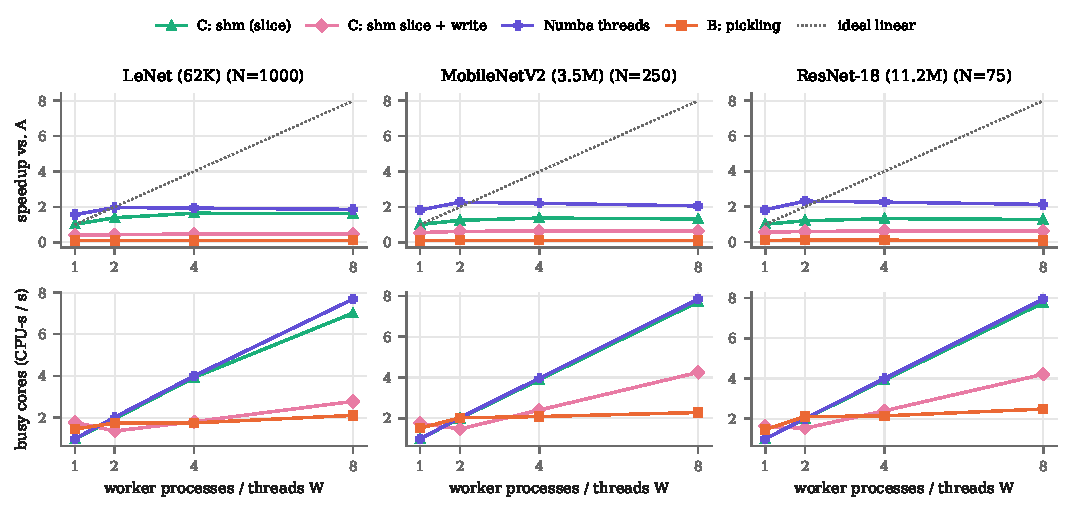
\includegraphics[width=\textwidth]{fig_scaling}
\caption{Scaling with worker count at the largest client count per model. Top: speedup over Scheme A (dotted: ideal linear speedup). Bottom: busy cores of the process tree. Cores become busy, but speedup saturates because aggregation is memory-bandwidth bound.}
\label{fig:scaling}
\end{figure*}

\begin{table}[t]
\caption{Speedup over Scheme A vs.\ Worker Count at the Largest $N$}
\label{tab:scaling}
\centering
\footnotesize
\setlength{\tabcolsep}{4pt}
\resizebox{\columnwidth}{!}{%
\begin{tabular}{@{}llrrrr@{}}
\toprule
Model ($N$) & Scheme & $W{=}1$ & $W{=}2$ & $W{=}4$ & $W{=}8$ \\
\midrule
\multirow{4}{*}{LeNet (1000)} & C: slice & 1.02 & 1.39 & \textbf{1.64} & 1.63 \\
 & C: slice + write & 0.39 & 0.43 & 0.47 & 0.46 \\
 & Numba & 1.56 & 1.96 & 1.93 & 1.86 \\
 & B: pickling & 0.10 & 0.11 & 0.11 & 0.11 \\
\midrule
\multirow{4}{*}{MobileNetV2 (250)} & C: slice & 1.01 & 1.24 & \textbf{1.37} & 1.32 \\
 & C: slice + write & 0.55 & 0.62 & 0.65 & 0.64 \\
 & Numba & 1.82 & 2.27 & 2.20 & 2.06 \\
 & B: pickling & 0.10 & 0.12 & 0.12 & 0.11 \\
\midrule
\multirow{4}{*}{ResNet-18 (75)} & C: slice & 1.01 & 1.20 & \textbf{1.32} & 1.27 \\
 & C: slice + write & 0.55 & 0.60 & 0.62 & 0.61 \\
 & Numba & 1.82 & 2.31 & 2.26 & 2.12 \\
 & B: pickling & 0.10 & 0.10 & 0.10 & 0.08 \\
\bottomrule
\end{tabular}}
\end{table}

\subsection{Partitioning Strategy}
Slice partitioning was faster than client partitioning in every configuration we measured (Fig.~\ref{fig:partition}), by 1.14--3.5$\times$ at $W=8$. The margin is largest where the reduction is most expensive relative to the work: at small $N$ on large models (3.5$\times$ for ResNet-18 at $N=10$, 3.3$\times$ for MobileNetV2 at $N=10$) and it narrows as $N$ grows (1.4$\times$ and 1.1$\times$ respectively at the largest $N$). The cause is structural: every worker writes a full $P$-length partial vector and the parent must then reduce $W$ such vectors sequentially, adding $W\!\cdot\!P$ of memory traffic that slice partitioning avoids entirely---and on a bandwidth-bound machine, added traffic is precisely what cannot be afforded.

This is a sharper result than the expectation we set out in Section~\ref{sec:method}. We anticipated that client partitioning would suit large $N$ and slice partitioning large $P$; in fact slice partitioning won everywhere, including on LeNet, where $N$ is largest relative to $P$ and where we had expected the two to be at worst equivalent. The anticipated advantage of client partitioning at large $N$ never materialised, and on a bandwidth-bound machine it is hard to see how it could: the strategy's defining cost is an extra $W\!\cdot\!P$ of traffic.

\begin{figure}[t]
\centering
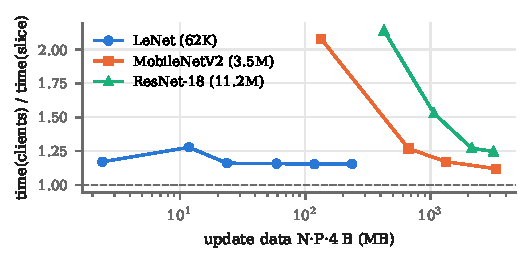
\includegraphics[width=\columnwidth]{fig_partition}
\caption{Time of client partitioning relative to slice partitioning in Scheme C ($W=8$). Values above 1 mean slice partitioning is faster; it is faster in every configuration measured.}
\label{fig:partition}
\end{figure}

\subsection{End-to-End Cost and Start-Up}
\label{sec:e2e}
The compute-only figures assume that updates already reside in shared memory. When the parent must first copy the $N$ received updates into the block, the end-to-end time is 1.8--3.5$\times$ the compute-only time (Table~\ref{tab:main}, ``C: slice + write''), and the result is unambiguous on this machine: end-to-end Scheme C \emph{never} beats the sequential baseline, in any configuration. The best case is 0.68$\times$ (MobileNetV2, $N=10$, $W=4$) and the largest configurations sit at 0.46--0.64$\times$. The reason is arithmetically simple and follows directly from Section~\ref{sec:rq3}: the single-threaded copy streams exactly the bytes the aggregation then reads, at the same single-core bandwidth the sequential baseline achieves, so it costs about as much as the parallel computation it enables, while the parallel part can recover at most the $\approx\!2\times$ the bus allows. On a bandwidth-bound machine, zero-copy aggregation is therefore not merely more efficient when updates arrive directly into shared memory---it is the only configuration in which the scheme is worth deploying at all. A server that deserialises client updates into private buffers and then copies them into a shared block should simply aggregate them sequentially.

Worker-pool start-up with \texttt{spawn} took 177--289\,ms, rising with $W$, an order of magnitude above the 12--28\,ms that \texttt{fork} achieves on Linux and well above the 64--98\,ms previously attributed to \texttt{spawn} platforms. Because the pool is created once and reused for every round, this is a one-off cost: amortised over a 20-round session it adds under 15\,ms per round, and over a realistic deployment it vanishes. It would, however, dominate entirely if a pool were created per round, which is the failure mode \texttt{spawn} makes easy to fall into.

\subsection{Summary of Hypotheses}
\textbf{H1} (shared memory outperforms sequential aggregation, with speedup increasing with $N$ and $P$ up to a plateau) is \emph{partially supported, and more weakly than anticipated}. Scheme C is faster once the update data exceeds roughly 12\,MB and slower below it, which is the predicted shape, but the magnitude is 1.09--1.64$\times$ rather than the hypothesised near-linear region, and the plateau arrives almost immediately: for MobileNetV2 the speedup moves only from 1.26$\times$ to 1.37$\times$ across a 25-fold increase in update volume. The prediction that speedup grows with $N$ and $P$ holds only in the narrow band below 236\,MB; beyond that the curve is flat. The hypothesis's rationale---that IPC overhead becomes negligible once the work is large---was correct but incomplete, because it assumed the arithmetic would then scale with $W$, and on this machine it cannot.

\textbf{H2} (shared memory outperforms pickling, with the margin growing with model size) is \emph{supported}: the margin grows from 5.4$\times$ at 2\,MB to 12--15$\times$ for the larger models, and Scheme B never beats the sequential baseline in any of the 56 configurations.

\textbf{H3} (speedup plateaus beyond an optimal worker count due to memory-bandwidth contention) is \emph{supported, and is the dominant effect in this study}: the optimum is $W=4$ for every model, efficiency falls to 0.17--0.20 at eight workers, and the STREAM measurement confirms the mechanism directly---one core already draws 9--12\,GB/s of a 21\,GB/s ceiling. We add one qualification the hypothesis did not anticipate: part of what looks like bus contention at high $W$ is in fact last-level-cache contention between the workers' private tiles, and is removable by sizing the tile for the aggregate of workers (Table~\ref{tab:tile}). The bandwidth wall is real, but it sits further out than the naive implementation suggests.

\subsection{Threats to Validity}
\label{sec:threats}
Results come from a single x86-64 Windows machine with \emph{single-channel} DDR5, and that last detail is the most important threat to external validity in this paper. Because the sequential baseline already consumes about half the available bandwidth, the headroom for any parallel scheme here is roughly $2\times$; on a dual- or quad-channel server with the same core count, the ceiling would be proportionally higher and Scheme C's speedups correspondingly larger. Our qualitative findings (B is catastrophic, slice beats clients, the optimum $W$ lies below the core count, the tile must be sized for the aggregate of workers) should transfer; the specific speedup magnitudes should not be read as properties of multi-process aggregation in general. Equally, behaviour under \texttt{fork} on Linux or on ARM/Apple Silicon with unified memory may differ, and results from different platforms must never be combined in one table or plot---an error we specifically avoided by discarding all earlier partial runs from other machines and re-measuring everything reported here in one sweep.

Timing noise was low: the inter-quartile range was a median of 2.1\% of the median and a 90th percentile of 14.2\%, though isolated configurations reached 53\%. We mitigated scheduler jitter with warm-up runs, shuffled interleaving, ten repetitions everywhere, mains power, the high-performance power plan, and closed background applications; no configuration was re-run or discarded. Synthetic updates are valid for timing but not for claims about model quality, which rest on the correctness track alone. Python-level overhead could affect the schemes differently; the shared kernel and the compiled Numba baseline limit this effect. Finally, the tile rule depends on detecting the last-level cache size, which we read from the OS and which could be wrong on an unusual topology; the rule degrades gracefully, since an underestimate merely yields a smaller tile and a 4--8\% loss rather than a collapse.

\section{Conclusion and Future Directions}
\subsection{Answers to the Research Questions}
We synthesize the empirical answers to our guiding questions as follows:
\begin{itemize}
\item \textbf{RQ1 (Speedup and Latency):} Multi-process shared-memory aggregation (Scheme C) achieves a 1.09--1.64$\times$ speedup over sequential FedAvg once update payloads exceed $\approx$12\,MB ($N \ge 50$ for LeNet, $N \ge 10$ for MobileNetV2 and ResNet-18). Below this threshold, fixed IPC metadata dispatch and barrier synchronization costs ($0.2$--$0.4$\,ms) overshadow arithmetic gains. The speedup saturates almost as soon as it appears, rather than growing with update volume.
\item \textbf{RQ2 (Data Movement Costs):} Explicit pickling and pipe transmission (Scheme B) is 5.6--21$\times$ slower than shared memory, never surpasses sequential aggregation in any of 56 configurations, and consumes up to 1.3\,GB of transient serialization memory against zero for shared memory. Zero-copy memory sharing is therefore an essential architectural requirement rather than an incremental optimization.
\item \textbf{RQ3 (Worker Scaling and Bandwidth Limits):} Scaling worker processes yields sub-linear speedups that peak at $W=4$ and decline thereafter, with parallel efficiency of 0.17--0.20 at $W=8$. Aggregation is fundamentally memory-bandwidth bound ($1/4$ FLOP/byte): the measured ceiling is 21\,GB/s, a single core already draws 9--12\,GB/s of it, and the available headroom is therefore about $2\times$ regardless of core count. A second, removable limit is last-level-cache contention between workers' private tiles, which a worker-count-aware tile eliminates, recovering up to 60\% of throughput at $W=8$.
\end{itemize}

We implemented and compared sequential, pickling-based, shared-memory, and multithreaded aggregation for federated learning on a commodity laptop, under one interface and one arithmetic kernel. All schemes are numerically equivalent, and shared-memory aggregation reproduces the sequential FedAvg result bit-for-bit on CIFAR-10 and FEMNIST. Shared memory reduces aggregation time by 1.09--1.64$\times$ once the update volume is non-trivial, and it is 5.6--21$\times$ faster than pickling-based multiprocessing, which never beats the sequential baseline.

The honest headline of this study, however, is a negative one with a positive corollary. On a single-channel commodity laptop, server-side FedAvg aggregation is so thoroughly memory-bandwidth bound that one core already saturates half the bus, and no amount of parallelism---processes or threads---can recover more than about $2\times$. Parallelising aggregation is therefore not where effort on such machines should go; reducing the bytes moved is. The corollary is that the two things which \emph{do} matter are architectural rather than arithmetic: never copy the updates (pickling costs an order of magnitude and zero-copy sharing is a precondition, not an optimisation), and size the kernel's cache tile for the aggregate of the workers rather than for one, since the natural fixed tile silently turns a speedup into a 2$\times$ slowdown at eight workers. In-process threads (Numba) were fastest in all 56 comparisons, so shared-memory multiprocessing is the right choice specifically where threads are not an option: Python code holding the global interpreter lock, sandboxed workers, or aggregator components that must run as separate processes.

Future work includes: (i)~repeating the study on a dual- or quad-channel server to separate the bandwidth ceiling from the architecture, and on ARM/Apple Silicon with unified memory, since this paper's magnitudes are a property of a single-channel machine; (ii)~receiving client updates from the network directly into shared memory, without which the end-to-end scheme never beats the sequential baseline at all; (iii)~lowering memory traffic with reduced-precision (float16/bfloat16) or compressed updates, which attacks the actual bottleneck rather than working around it; (iv)~combining shared memory with threads or Numba inside each worker, and pinning workers to cores; and (v)~integrating the aggregator into a full FL framework and evaluating it with real FedScale device traces and secure aggregation.

\begin{thebibliography}{99}
\bibitem{fedscale} F. Lai, Y. Dai, S. S. Singapuram, J. Liu, X. Zhu, H. V. Madhyastha, and M. Chowdhury, ``FedScale: Benchmarking model and system performance of federated learning at scale,'' in \emph{Proc. 39th Int. Conf. Machine Learning (ICML)}, PMLR 162, pp. 11814--11827, 2022.
\bibitem{p2pfed} A. Lim, S. Jang, and J. Lee, ``P2P-Fed: A decentralized federated learning platform on structured peer-to-peer systems,'' in \emph{Proc. IEEE 25th Int. Symp. Cluster, Cloud and Internet Computing (CCGrid)}, pp. 124--133, 2025.
\bibitem{gain} J. Xia, W. Wu, L. Luo, G. Cheng, D. Guo, and Q. Nian, ``Accelerating and securing federated learning with stateless in-network aggregation at the edge,'' in \emph{Proc. IEEE 44th Int. Conf. Distributed Computing Systems (ICDCS)}, pp. 692--702, 2024.
\bibitem{flagger} X. Pan, Y. An, S. Liang, B. Mao, M. Zhang, Q. Li, M. Jung, and J. Zhang, ``Flagger: Cooperative acceleration for large-scale cross-silo federated learning aggregation,'' in \emph{Proc. 51st ACM/IEEE Int. Symp. Computer Architecture (ISCA)}, pp. 915--930, 2024.
\bibitem{jiang2022} Z. Jiang, W. Wang, B. Li, and Q. Yang, ``Towards efficient synchronous federated training: A survey on system optimization strategies,'' \emph{IEEE Trans. Big Data}, 2022.
\bibitem{khan2023} A. F. Khan, M. F. A. Shahid, M. H. U. Rehman, and S. U. Khan, ``Towards cost-effective and resource-aware aggregation at edge for federated learning,'' in \emph{Proc. IEEE 19th Int. Conf. e-Science (e-Science)}, pp. 1--10, 2023.
\bibitem{lifl} S. Qi, K. K. Ramakrishnan, and M. Lee, ``LIFL: A lightweight, event-driven serverless platform for federated learning,'' in \emph{Proc. MLSys}, 2024.
\bibitem{falkor} M. Georgieva Belorgey, S. Dandjee, N. Gama, D. Jetchev, and D. Mikushin, ``Falkor: Federated learning secure aggregation powered by AES-CTR GPU implementation,'' in \emph{Proc. WAHC @ ACM CCS}, 2023.
\bibitem{mcmahan2017} B. McMahan, E. Moore, D. Ramage, S. Hampson, and B. A. y Arcas, ``Communication-efficient learning of deep networks from decentralized data,'' in \emph{Proc. 20th Int. Conf. Artificial Intelligence and Statistics (AISTATS)}, PMLR 54, pp. 1273--1282, 2017.
\bibitem{numba} S. K. Lam, A. Pitrou, and S. Seibert, ``Numba: A LLVM-based Python JIT compiler,'' in \emph{Proc. 2nd Workshop on the LLVM Compiler Infrastructure in HPC (LLVM '15)}, pp. 1--6, 2015.
\bibitem{numpy} C. R. Harris \emph{et al.}, ``Array programming with NumPy,'' \emph{Nature}, vol. 585, pp. 357--362, 2020.
\bibitem{pyshm} Python Software Foundation, ``\texttt{multiprocessing.shared\_memory} --- Shared memory for direct access across processes,'' \emph{Python 3 Documentation}. [Online]. Available: \url{https://docs.python.org/3/library/multiprocessing.shared_memory.html}
\bibitem{pytorch} A. Paszke \emph{et al.}, ``PyTorch: An imperative style, high-performance deep learning library,'' in \emph{Advances in Neural Information Processing Systems (NeurIPS)}, vol. 32, 2019.
\bibitem{flower} D. J. Beutel \emph{et al.}, ``Flower: A friendly federated learning research framework,'' arXiv:2007.14390, 2020.
\bibitem{lenet} Y. LeCun, L. Bottou, Y. Bengio, and P. Haffner, ``Gradient-based learning applied to document recognition,'' \emph{Proc. IEEE}, vol. 86, no. 11, pp. 2278--2324, 1998.
\bibitem{cifar} A. Krizhevsky, ``Learning multiple layers of features from tiny images,'' Tech. Rep., University of Toronto, 2009.
\bibitem{hsu2019} T.-M. H. Hsu, H. Qi, and M. Brown, ``Measuring the effects of non-identical data distribution for federated visual classification,'' arXiv:1909.06335, 2019.
\bibitem{leaf} S. Caldas \emph{et al.}, ``LEAF: A benchmark for federated settings,'' arXiv:1812.01097, 2018.
\bibitem{mobilenetv2} M. Sandler, A. Howard, M. Zhu, A. Zhmoginov, and L.-C. Chen, ``MobileNetV2: Inverted residuals and linear bottlenecks,'' in \emph{Proc. IEEE/CVF Conf. Computer Vision and Pattern Recognition (CVPR)}, pp. 4510--4520, 2018.
\bibitem{resnet} K. He, X. Zhang, S. Ren, and J. Sun, ``Deep residual learning for image recognition,'' in \emph{Proc. IEEE Conf. Computer Vision and Pattern Recognition (CVPR)}, pp. 770--778, 2016.
\bibitem{stream} J. D. McCalpin, ``Memory bandwidth and machine balance in current high performance computers,'' \emph{IEEE Computer Society Technical Committee on Computer Architecture (TCCA) Newsletter}, vol. 1995, no. 12, pp. 19--25, Dec. 1995.
\end{thebibliography}

\end{document}
